\documentclass[11pt a4paper]{article}
\usepackage[margin=2cm]{geometry}
\usepackage{amsmath, amssymb}
\usepackage{graphicx}
\usepackage{float}
\usepackage{aligned-overset}
\usepackage{subcaption}
\usepackage{tabularx} % fuer gleichungen nebeneinander
\usepackage{wrapfig} % damit figures neben text sien koennen

% partielle ableitungen
\newcommand{\delr}{\partial_r}
\newcommand{\delt}{\partial_t}
\newcommand{\deltheta}{\partial_\theta}
\newcommand{\delphi}{\partial_\varphi}

% elektrische feldkonstante
\newcommand{\epsz}{\epsilon_0}
% 1 / 4pi eps
\newcommand{\kco}{\frac{1}{4\pi\epsilon_0}}
% del fuer partial
\newcommand{\del}{\partial}

% div und rot
\newcommand{\diver}{\vec \nabla \cdot}
\newcommand{\rot}{\vec \nabla \times}
\newcommand{\grad}{\vec \nabla}

% hyperbolische funktionen
\newcommand{\arsinh}{\text{arsinh}}
\newcommand{\arcosh}{\text{arcosh}}
\newcommand{\artanh}{\text{artanh}}

% fuer impedanzen 
\newcommand{\omegaC}{\omega C}
\newcommand{\omegaL}{\omega L}
\newcommand{\omegaR}{\omega R}
\newcommand{\omegaLC}{\omega LC}
\newcommand{\omegaLCR}{\omega LCR}
\newcommand{\omegaCR}{\omega CR}

% fancy header
\usepackage{fancyhdr}
\fancyhf{}
% vspaces in den headern fuer Distanzen notwendig
% linke Seite: Namen der Abgabegruppe
\lhead{\textbf{Matthias Maile\\Roman Surma}\vspace{1.5cm}}
% rechte Seite: Modul, Gruppe, Semester
\rhead{\textbf{Physik II - Gruppe 2\\Sommersemester 2020}\vspace{1.5cm}}
% Center: nr. des blattes
\chead{\vspace{2.5cm}\huge{\textbf{23. Übungsblatt}}}
% benoetigt damit der eigentliche Text nicht in der Überschrift steckt
\setlength{\headheight}{4cm}

% zum zeichnen tikz
\usepackage{tikz}

% fuer fabigen text
\usepackage{xcolor}

% irgendwas mit figures
\usepackage{subcaption}

\begin{document}
\thispagestyle{fancy}

\section*{Aufgabe 1}
\[ \vec E = E_0 \vec e_y \cdot \cos(kx - \omega t) \]
a) Ausbreitung in $x$-Richtung $\Rightarrow \vec k = k \cdot \vec e_x $ \\
Damit folgt $\vec B$:
\begin{align*}
	\vec B = \frac{\vec k \times \vec E}{\omega} 
	&= \underbrace{\frac{k}{\omega} \cdot E_0}_{B_0 = \frac{E_0}{c}}
		\cdot (\vec e_x \times \vec e_y) \cdot \cos(kx - \omega t) \\
	&= \underbrace{B_0 \cdot \vec e_z}_{\vec B = B_0 \vec e_z} \cdot \cos(kx - \omega t) \\
\end{align*}
% berechnung des poynting vektors
\begin{align*}
	\vec S = \frac{\vec E \times \vec B}{\mu_0}
	&= \frac{E_0 \cdot B_0}{\mu_0} \cdot \cos^2(kx - \omega t) \cdot (\vec e_y \times \vec e_z) \\
	&= \frac{E_0 \cdot B_0}{\mu_0} \cdot \cos^2(kx - \omega t) \cdot \vec e_x \\
	&= \frac{E_0^2}{c \mu_0} \cdot \cos^2(kx - \omega t) \cdot \vec e_x \\
\end{align*}
b) Der Poynting-Vektor zeigt in die Richtung des Energieflusses und der Betrag von diesem ist die Intensität des 
Energieflusses zum Zeitpunkt $t$.

\vspace{0.5cm}
\noindent 
c)
\begin{align*}
	I = \langle \vert \vec s \vert \rangle_t 
	&= \frac{E_0^2}{c\mu_0} \langle \vert \cos^2(kx - \omega t) \vert \rangle_t
	&= \frac{E_0^2}{2c\mu_0}
\end{align*}

\vspace{0.5cm}
\noindent 
d)
\[ P = \frac{I}{c} = \frac{E_0^2}{2c^2\mu_0} = \frac{B_0^2}{2\mu_0} \]
e) 
\[ P = \frac{I}{c} = \frac{1.4 \cdot 10^3 \ Wm^{-2}}{3 \cdot 10^8 m/s} \approx 4.67 \cdot 10^{-6} Nm^{-2} 
\Rightarrow 
F = PA = P \cdot \pi R_E^2 \approx 5.95 \cdot 10^{8} \ N 
\]

\newpage
\setlength{\headheight}{0cm}

\section*{Aufgabe 2}
\par{a)} Beim ersten Fall entsteht eine linear polarisierte Welle:
\begin{itemize}
	\item $\delta = 0: \ \vec E 
		= \begin{pmatrix} \vert \hat E_x \vert \cdot \cos(kz - \omega t)  \\
		\vert \hat E_y \vert \cdot \cos(kz - \omega t) \end{pmatrix}
		= \cos(kz - ω t) \cdot \begin{pmatrix} \vert \hat E_x \vert \\ \vert \hat E_y \vert \end{pmatrix}$
	\item $\delta = \pm\pi: \ \vec E 
		= \begin{pmatrix} \vert \hat E_x \vert \cdot \cos(kz - \omega t)  \\ 
			\vert \hat E_y \vert \cdot \cos\left(kz - \omega t \pm \pi \right)  \end{pmatrix}
		% cos in sin umschreiben
		= \begin{pmatrix} \vert \hat E_x \vert \cdot \cos(kz - \omega t)  \\ 
			-\vert \hat E_y \vert \cdot \cos\(kz - \omega t)  \end{pmatrix}
		= \cos\left(kx - \omega t\right) \begin{pmatrix} \vert \hat E_x \vert \\ 
			-\vert \hat E_y \vert \ \end{pmatrix}
			$
\end{itemize}
Beim zweiten Fall entsteht eine elliptisch polarisierte Welle (da $\vert \hat E_x \vert \neq \vert \hat E_y \vert$ keine zirkular polarisierte Welle):
\begin{align*}
	\vec E 
	&= \begin{pmatrix}
		\vert \hat E_x \vert \cdot \cos(kz - \omega t) \\
		\vert \hat E_y \vert \cdot \cos(kz - \omega t \pm \frac\pi2) \\
	\end{pmatrix} 
	= \begin{pmatrix}
		\vert \hat E_x \vert \cdot \cos(kz - \omega t) \\
		\mp \vert \hat E_y \vert \cdot \sin(kz - \omega t) \\
	\end{pmatrix}
\end{align*}

\begin{figure}[H]
	\centering
	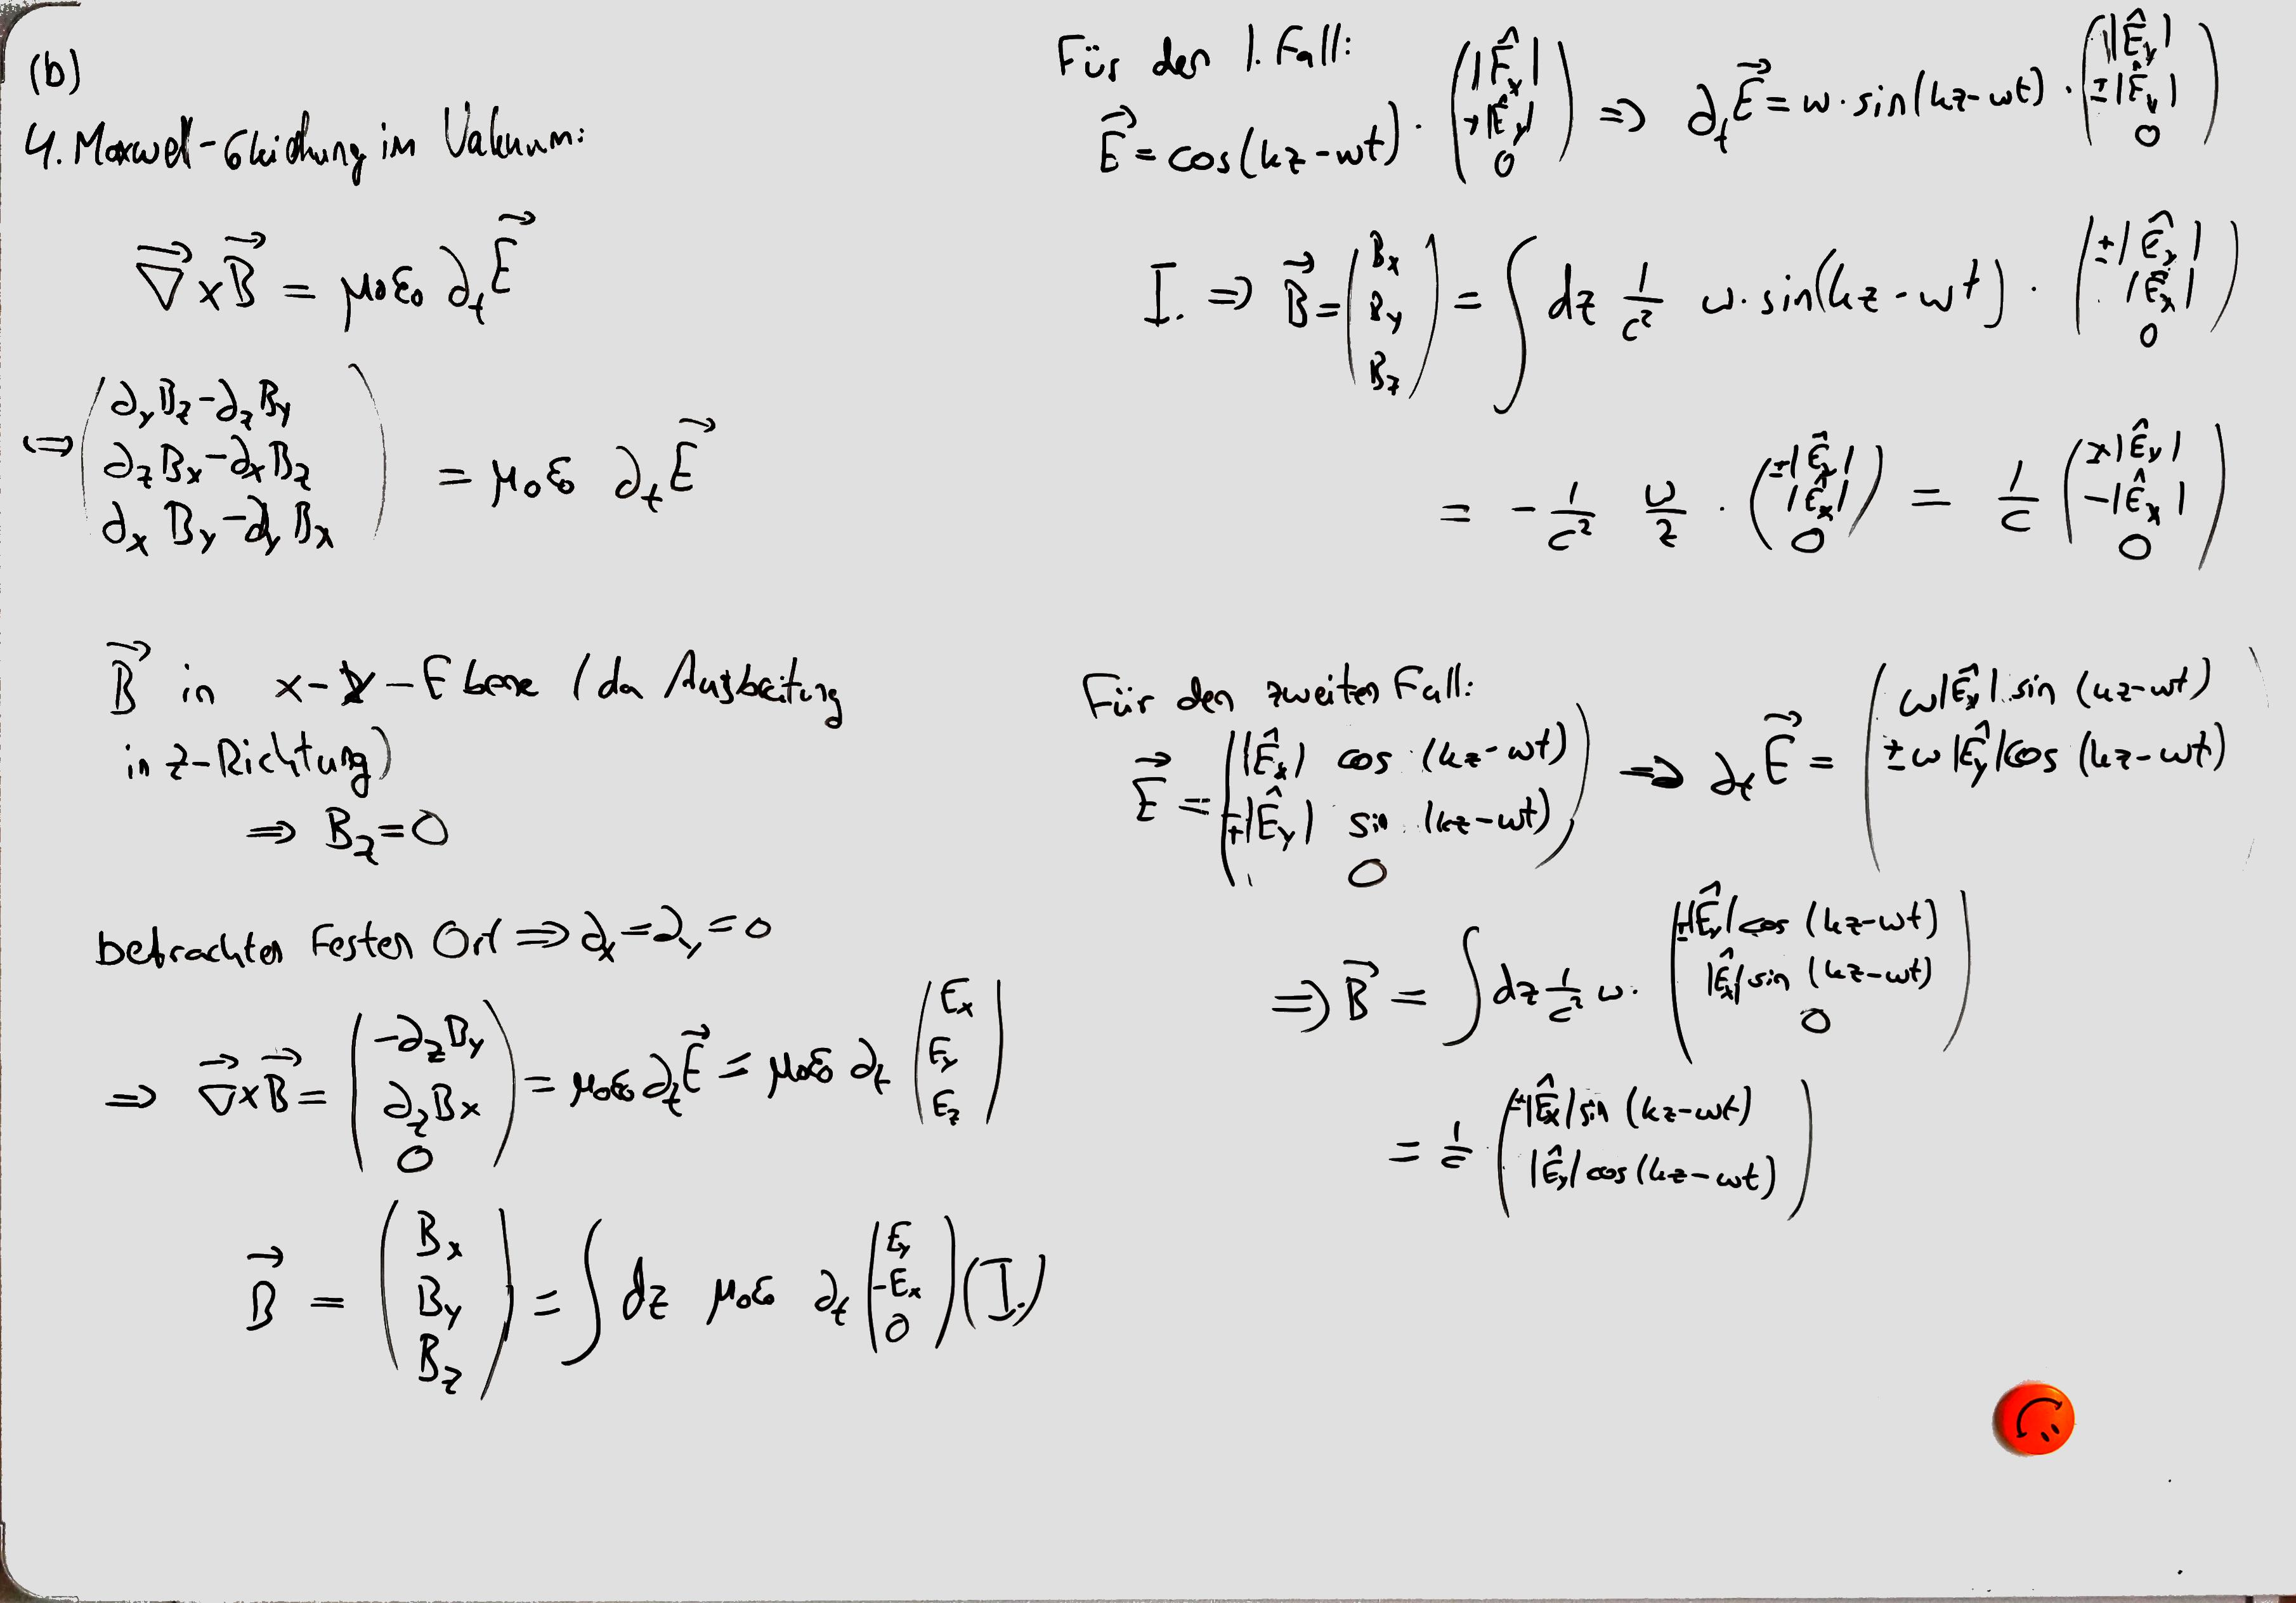
\includegraphics[width=18cm]{aufgabe2b.jpg}
\end{figure}

\newpage

\section*{Aufgabe 3}

\begin{figure}[H]
	\centering
	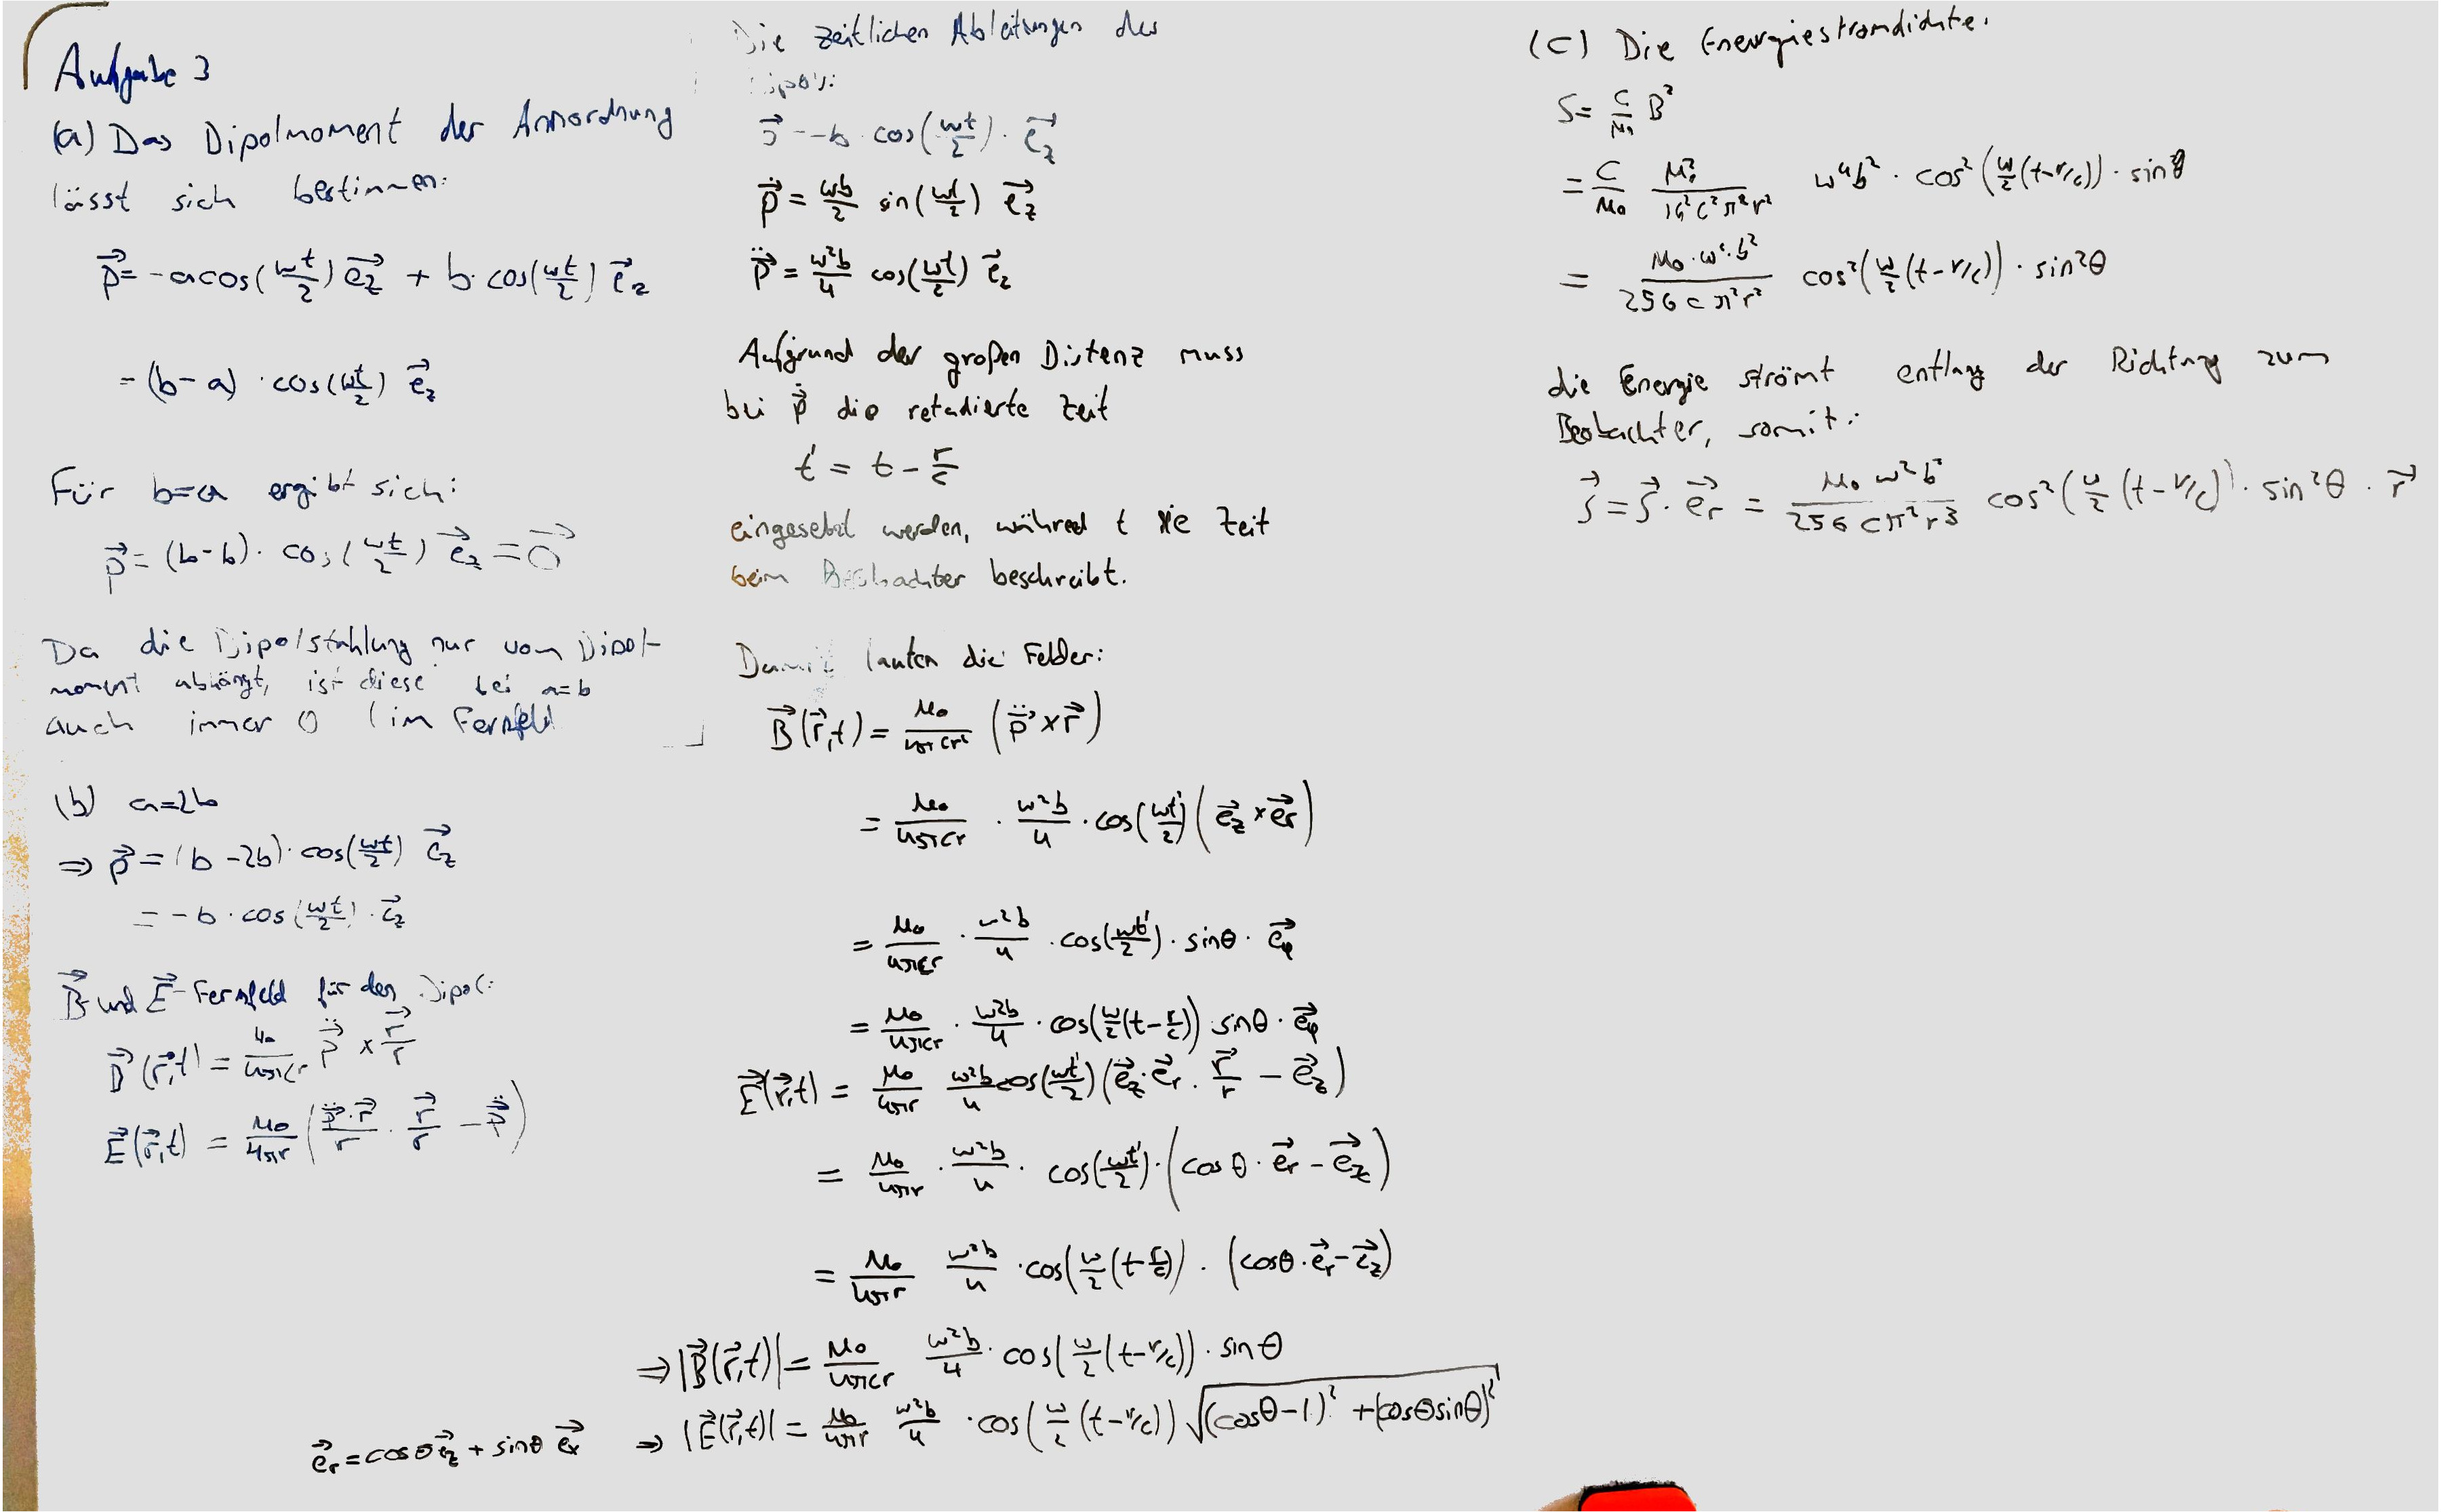
\includegraphics[width=18cm]{aufgabe3.jpg}
\end{figure}

\newpage

\section*{Aufgabe 4}
\par{a)} Auf das Elektron wirkt eine Lorentzkraft, wodurch zum Zeitpunk $t_0 + \Delta t$ das Elektron nicht mehr
in die gleiche Richtung fliegt. \\
Waere $\vec v (0) = v_0 \vec e_x$, so gaebe es zum spaeteren Zeitpunkt eine Komponente in $y$-Richtung.

Da das Elektron auf einer Kreisbahn ist wirken Scheinkraefte. Daher ist das Ruhesystem des Elektrons kein
Inertialsystem.

\end{document}
